\documentclass[10pt, a4paper]{article}
\usepackage{enumerate, listings, enumitem, etoolbox}
\usepackage[spanish]{babel}
%\usepackage{a4wide} % márgenes un poco más anchos que lo usual
\usepackage{fullpage}
\usepackage[utf8]{inputenc}
\usepackage{aed2-symb,aed2-itef,aed2-tad,aed2-diseno}
\usepackage{color} % para snipets de codigo coloreados
\usepackage{fancybox}  % para el sbox de los snipets de codigo
\usepackage[paper=a4paper, left=1.5cm, right=1.5cm, bottom=1.5cm, top=3.5cm]{geometry}
\usepackage[utf8]{inputenc}
\usepackage[T1]{fontenc}
\usepackage[spanish]{babel}
\usepackage{indentfirst}
\usepackage{fancyhdr}
\usepackage{latexsym}
\usepackage{lastpage}
\usepackage[colorlinks=true, linkcolor=blue]{hyperref}
\usepackage{calc}
\usepackage{algorithmicx, algorithm}
% \usepackage[noend]{algpseudocode} % deshabilita end if, endwhile, endfor
\usepackage{algpseudocode}
\usepackage{xcolor}
\usepackage{enumerate, listings, enumitem, etoolbox}
\usepackage{pdfpages}
\usepackage{tikz}

\newcommand{\bigO}{\mathcal{O}}
\newcommand{\asignar}[2]{$#1 \gets #2$}
\algrenewcommand\alglinenumber[1]{\tiny #1:}  % Para que los numeros de linea del pseudo sean pequeños
\renewcommand{\thealgorithm}{}  % Que no aparezca el numero luego de "Algorithm"
\floatname{algorithm}{ }    % Entre {  } que quiero que aparezca en vez de "Algorithm"

\parskip=5pt % 10pt es el tamaño de fuente
\parindent=0pt

\begin{document}

\thispagestyle{empty}
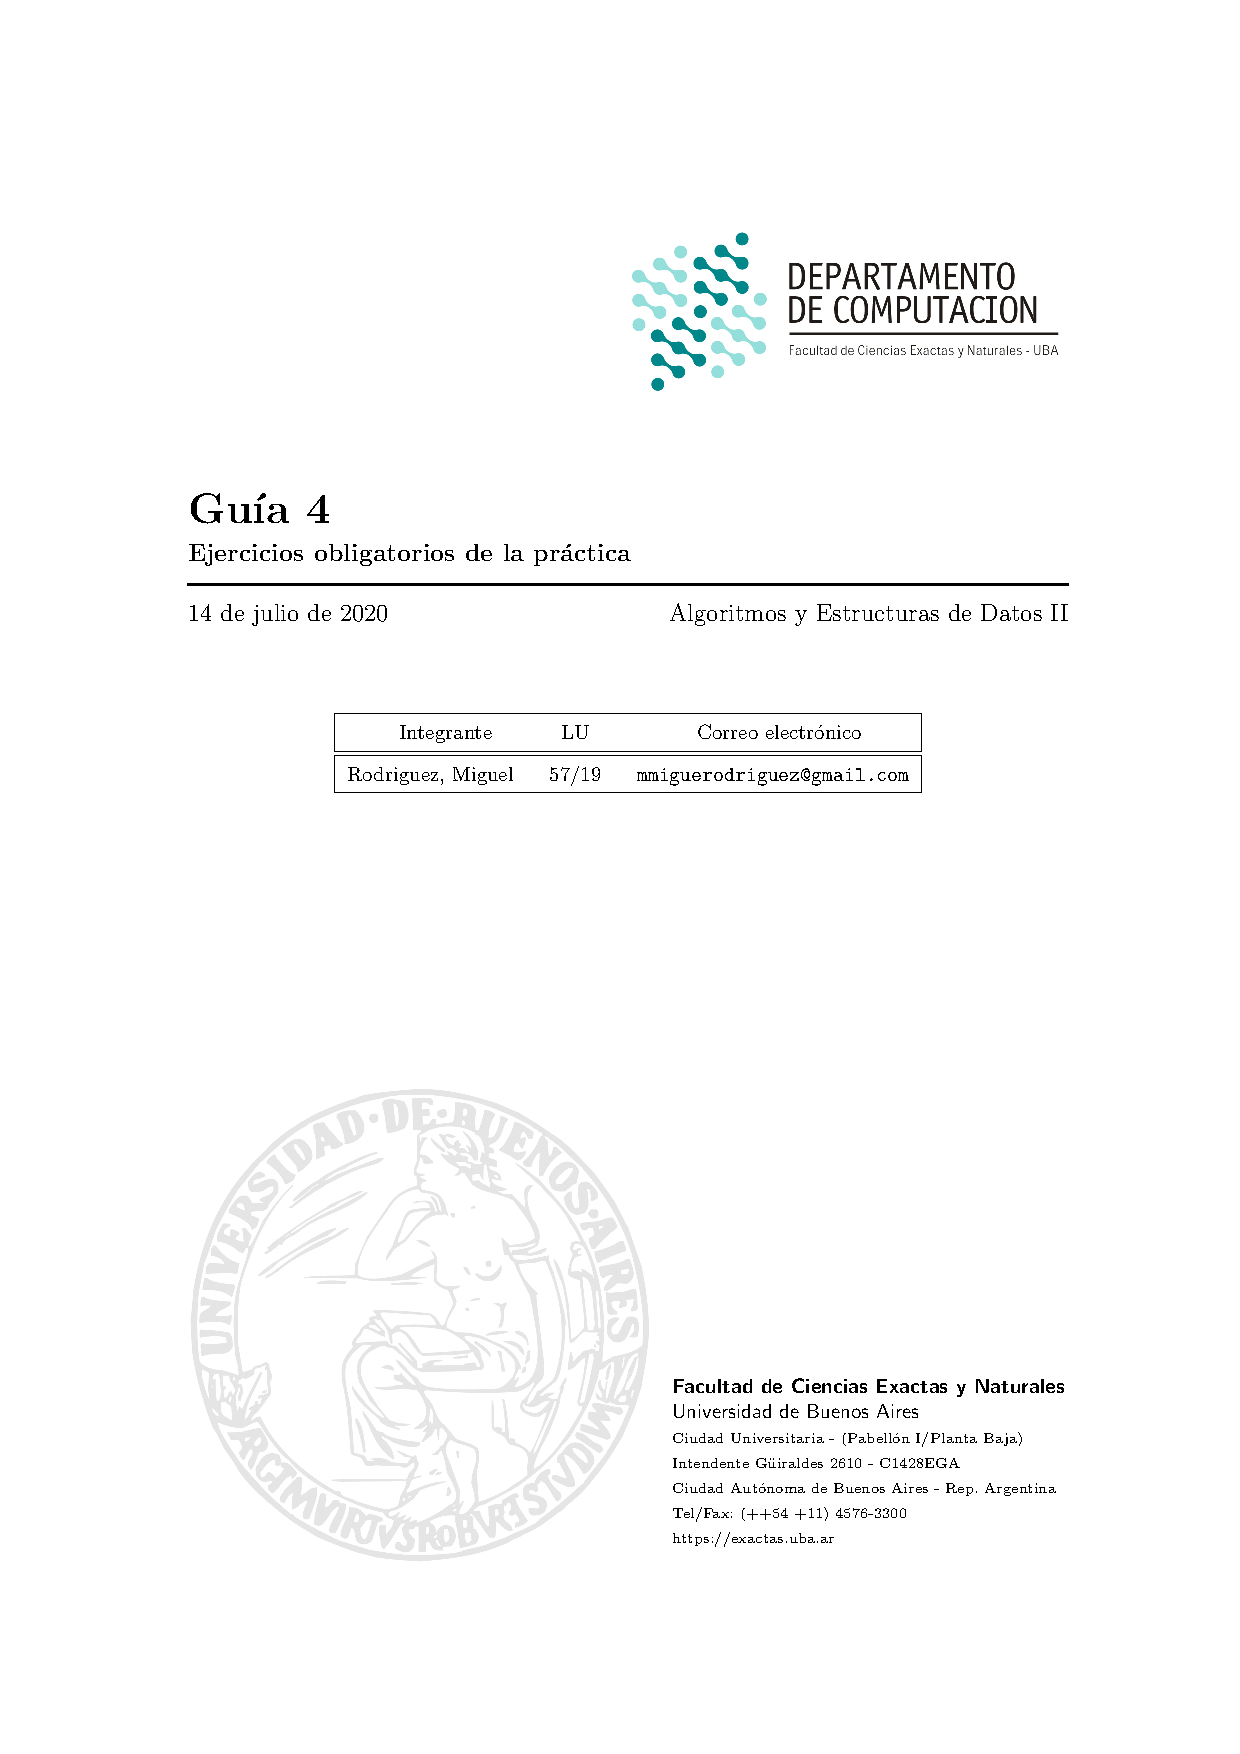
\includepdf[pages=-,pagecommand={},width=\textwidth]{include/caratula.pdf}

\setcounter{page}{1}

\section*{Ejercicio 1: Ordenamiento}
Se tiene un arreglo $A$ de $N$ conjuntos $A[1],...,A[N]$. El cardinal de cada conjunto es \textbf{a lo sumo} $K$, es decir \#$(A[i])\leq K$ para todo $1 \leq i \leq N$. Se desea ordenar el arreglo $A$ para obtener como resultado un arreglo de conjuntos $B[1],...,B[N]$ de tal modo que se cumpla con la siguiente condicion:
\begin{center}
$B[i] \subseteq B[j] \implies i \leq j$ \tab para todo $i,j$ en el rango $1..N$
\end{center}
es decir, si un conjunto est\'a incluido en otro, debe aparecer antes en el arreglo ordenado.

\vspace{0.5em}

\textbf{Idea: }
\begin{enumerate}
  \item Armar un bucket en el que vamos a guardar los conjuntos o sus iteradores seg\'un sus cardinales.
  \item A partir de los buckets, armar una lista ordenada por el cardinal de los conjuntos, ya que, si est\'an ordenados por tama\~no, necesariamente se va a cumplir la condici\'on de que si un conjunto est\'a incluido en el otro, su \'indice va a ser menor.
\end{enumerate}

\textbf{Algoritmo: }
\begin{enumerate}
  \item Los \texttt{conj(nat)} dentro del vector recibido por par\'ametro est\'an representados por el m\'odulo \textsc{ConjuntoDeNaturales}.
  \item Lo primero que hacemos es generar un \texttt{vector(vector(itConj(nat)))} en el que el tama\~no del vector va a ser $K$, y el tama\~no de los vectores internos va a ser la cantidad de conjuntos que su cardinal sea el \'indice. Esto va a funcionar como nuestro "bucket". Suponemos que podemos recibir conjuntos con cardinal = 0.
  \item Una vez generado este vector, para calcular el resultado insertamos en el \texttt{vector(conj(nat))} una copia de cada conjunto a partir de su iterador. Suponemos en este caso que tenemos una funci\'on $copy(itConj)$ que a partir de un iterador de \textsc{ConjuntoDeNaturales} retorna una copia de la misma representaci\'on en tiempo lineal.
\end{enumerate}

\begin{algorithm}[H]
	\caption{\textbf{ordenarConjuntos}(\In{A}{vector(conj(nat))}, \In{k}{nat}) $\to$ $res$ : \texttt{vector(conj(nat))}}
	\begin{algorithmic}[1]
			\State \asignar{bucket}{Vacia()}
      \State \asignar{i}{0}
      \While{$i \leq k$} \Comment{$\bigO(K)$}
        \State $AgregarAtras(bucket, Vacia())$
        \State \asignar{i}{i + 1}
      \EndWhile
      \For{$a$ \textbf{in} $A$} \Comment{$\bigO(N \cdot K)$}
        \State \asignar{it}{CrearIt(a)} \Comment{$\bigO(1)$}
        \State $AgregarAtras(bucket[cardinal(a)], it)$ \Comment{$\bigO(K)$}
      \EndFor
      \State \asignar{res}{Vacia()}
      \State \asignar{i}{0}
      \While{$i \leq k$} % \Comment{$\bigO(K)$}
        \For{$a$ \textbf{in} $bucket[i]$} \Comment{Peor caso, un bucket tiene todos los conjuntos. $\bigO(N)$}
          \State $AgregarAtras(res, copy(a))$ \Comment{En total se va a ejecutar N veces. $\bigO(K)$}
        \EndFor
        \State \asignar{i}{i + 1}
      \EndWhile
      \State \Return{res}
			\medskip
	\end{algorithmic}
\end{algorithm}

\begin{algorithm}[H]
	\caption{\textbf{cardinal}(\In{A}{conj(nat)}) $\to$ $res$ : \texttt{nat}}
	\begin{algorithmic}[1]
      \State \asignar{i}{0}
      \For{$a$ \textbf{in} $A$} \Comment{$\bigO(\#(A))$}
        \State \asignar{i}{i + 1}
      \EndFor
      \State \Return{i}
			\medskip
	\end{algorithmic}
\end{algorithm}

\textbf{Complejidad: }
\begin{enumerate}
  \item Crear un \texttt{vector(vector(itConj(nat)))} de tama\~no $K$ nos cuesta $\bigO(K)$.
  \item Iterar por todos los elementos de la lista de entrada $A$ de tama\~no $N$, calcular el cardinal de cada uno, y devolver su iterador en cada paso nos cuesta $\bigO(N \cdot K)$.
  \item Iterar por el bucket, en principio pareciera que nos cuesta un tiempo cuadr\'atico, pero esto no ocurre, ya que en los buckets vac\'ios no se van a realizar operaciones, podemos tomarlas como $\bigO(1)$.
  \item La l\'inea 15, que inserta un conjunto en el vector de resultado se va a ejecutar exactamente $N$ veces, y en cada una el costo va a depender de $i$, ya que, son la cantidad de elementos a insertar (copiar) en el arreglo de salida. En peor caso, se va a ejecutar las $N$ veces con $i = K \implies \bigO(N \cdot K)$.
\end{enumerate}

Por lo explicado anteriormente y por el hecho de que $AgregarAtras$ se va a ejecutar siempre exactamente $N$ veces y su costo es a lo sumo $\bigO(K)$, queda demostrado que \textsc{ordenarConjuntos} $\in \bigO(N \cdot K)$. $\blacksquare$

\section*{Ejercicio 2: Dividir y conquistar}

Se tiene un arreglo $C$ de $N$ conjuntos $C[1],...,C[N]$. El cardinal de cada conjunto es \textbf{exactamente} $M$, es decir \#$(C[i]) = M$ para todo $1 \leq i \leq N$.

\textbf{1.} Proponer un algoritmo para determinar si los conjuntos $C[1],...,C[N]$ son disjuntos dos a dos, es decir si para todo $i \neq j$ en el rango $1...N$ se tiene que $C[i] \cap C[j] = \emptyset$. La complejidad temporal en peor caso del algoritmo debe ser $O(M \cdot N \cdot \log N)$. Justificar la complejidad temporal obtenida.

\vspace{0.5em}

\textbf{Idea: }
\begin{enumerate}
  \item Por la forma en la que se puede iterar el m\'odulo \textsc{ConjuntoDeNaturales}, podemos pensar que tenemos una lista grande de tama\~no $N$, que adentro, tiene listas ordenadas de exactamente $M$ elementos.
  \item Mi idea es parecida al funcionamiento de un Merge Sort, ya que, estaremos dividiendo el arreglo de conjuntos en partes mas chicas, y al resultado de cada divisi\'on (que va a estar ordenada), la unimos de forma ordenada.
  \item Una vez que tenemos todos los elementos ordenados, lo unico que resta hacer es revisar que no hayan elementos repetidos, ya que si se encuentra alg\'un repetido, quiere decir que hay m\'as de un conjunto que contiene ese elemento (por el hecho de ser conjuntos y que no pueden tener repetidos) y significa que no todos los conjuntos son disjuntos dos a dos.
\end{enumerate}

\textbf{Algoritmo: }
\begin{enumerate}
  \item Mi forma de realizar el algoritmo parte en dividir en mitades el arreglo de tama\~no $N$, por lo que vamos a tener $\log N$ niveles o llamadas recursivas.
  \item El caso base, sera cuando los \'indices $start$ y $end$ sean iguales, por lo que vamos a tener un solo conjunto, en ese caso, me armo un nuevo vector e inserto todos sus elementos. Esto nos cuesta exactamente $\Theta(M)$ ya que insertar en un vector es $\bigO(1)$ e iterar por un \'unico conjunto de exactamente $M$ elementos nos cuesta $\bigO(M)$. Notar que este vector va a estar ordenado por la forma en la que se itera un \textsc{ConjuntoDeNaturales}.
  \item Para la parte de dividir, llamo recursivamente a la funci\'on \textsc{sonDisjuntosAux} y as\'i obtengo las dos mitades ordenadas ya no como un conjunto sino como un \texttt{vector(nat)}.
  \item El paso de conquistar, es cuando hacemos el merge de las dos mitades ordenadas, que en tiempo lineal, nos va a retornar la uni\'on ordenada. El costo de copia por el pasaje de los par\'ametros est\'a acotado por la complejidad de la funci\'on.
  \item Finalmente, a partir del resultado de la funci\'on \textsc{hayRepetidos} decidimos si los conjuntos son disjuntos dos a dos.
\end{enumerate}

\begin{algorithm}[H]
	\caption{\textbf{sonDisjuntos}(\In{A}{vector(conj(nat))}) $\to$ $res$ : \texttt{bool}}
	\begin{algorithmic}[1]
			\State \asignar{resVector}{sonDisjuntosAux(a, 0, Longitud(a) - 1)} \Comment{$\bigO(N \cdot M \cdot \log N)$}
      \State \asignar{res}{\neg hayRepetidos(resVector)} \Comment{$\bigO(N \cdot M)$}
      \State \Return{res}
			\medskip
	\end{algorithmic}
\end{algorithm}

\begin{algorithm}[H]
	\caption{\textbf{sonDisjuntosAux}(\In{A}{vector(conj(nat))}, \In{start}{nat}, \In{end}{nat}) $\to$ $res$ : \texttt{vector(nat)}}
	\begin{algorithmic}[1]
			\If{start = end}
        \State \asignar{res}{Vacia()}
        \For{$x$ \textbf{in} $a[start]$} \Comment{$\bigO(M)$}
          \State $AgregarAtras(res, x)$ \Comment{$\bigO(1)$}
        \EndFor
      \EndIf
      \State \asignar{half}{(end + start)/2}
      \State \asignar{s1}{sonDisjuntosAux(a, start, half)} \Comment{$T(\frac{N}{2})$}
      \State \asignar{s2}{sonDisjuntosAux(a, half + 1, end)} \Comment{$T(\frac{N}{2})$}
      \State \asignar{res}{merge(s1, s2)} \Comment{$\bigO(N \cdot M)$}
      \State \Return{res}
			\medskip
	\end{algorithmic}
\end{algorithm}

\begin{algorithm}[H]
	\caption{\textbf{merge}(\In{A}{vector(nat)}, \In{B}{vector(nat)}) $\to$ $res$ : \texttt{vector(nat)}}
	\begin{algorithmic}[1]
    \State \asignar{res}{Vacia()}
    \State \asignar{i}{0}
    \State \asignar{j}{0}
    \State \asignar{k}{Longitud(A) + Longitud(B)}
    \While{$i < k$} \Comment{$\bigO(|A| + |B|)$}
      \If{$j \geq Longitud(B) \lor (i < Longitud(A) \land A[i] < B[i])$}
        \State $AgregarAtras(res, A[i])$ \Comment{$\bigO(1)$}
        \State \asignar{i}{i + 1}
      \Else
        \State $AgregarAtras(res, B[j])$ \Comment{$\bigO(1)$}
        \State \asignar{j}{j + 1}
      \EndIf
      \State \asignar{k}{k + 1}
    \EndWhile
    \State \Return{res}
		\medskip
	\end{algorithmic}
\end{algorithm}

\begin{algorithm}[H]
	\caption{\textbf{hayRepetidos}(\In{A}{vector(nat)}) $\to$ $res$ : \texttt{vector(nat)}}
	\begin{algorithmic}[1]
    \State \asignar{i}{0}
    \For{$i < Longitud(A) - 1$} \Comment{$\bigO(|A|)$}
      \If{$A[i] = A[i + 1]$}
        \State \Return{true}
      \EndIf
      \State \asignar{i}{i + 1}
    \EndFor
    \State \Return{false}
		\medskip
	\end{algorithmic}
\end{algorithm}

\textbf{Complejidad:}
En principio, si tengo que escribir la complejidad como una recurrencia, podemos notar que el caso base es cuando $N = 1$. En este caso, solamente tenemos que recorrer el \'unico conjunto que hay de tama\~no $M \implies \Theta(M)$. Para $N > 1$ el caso es distinto, ya que tenemos una funci\'on recursiva que divide problema en dos mitades (el arreglo de tama\~no $N$) y adem\'as con el resultado de estas llamadas recursivas, realiza un merge en $\bigO(\frac{M \cdot N}{2} + \frac{M \cdot N}{2}) \in \bigO(M \cdot N)$ ya que tenemos que tener en cuenta que cada mitad tiene $\frac{M \cdot N}{2}$ elementos. La recurrencia a la que llego es:
\[
T(N) = \left\{\begin{array}{lcc}
    \Theta(M) &   si  & N = 1 \\
    \\ 2 \cdot T(\frac{N}{2}) + \bigO(N \cdot M)  & si  & N > 1
    \end{array}\right.
\]

Para demostrar que efectivamente esta complejidad es la pedida por el ejercicio, lo solucionaremos como una recurrencia t\'ipica.
Veamos los par\'ametros que requiere la demostraci\'on:
\begin{enumerate}
  \item $a = 2$. Cantidad de subproblemas a resolver.
  \item $b = M.$ Costo de uni\'on.
  \item $c = 2$. Particiones del problema.
  \item $d = \log_{c} a = 1$.
\end{enumerate}
Demostrando con la soluci\'on de la recurrencia t\'ipica\footnote{https://campus.exactas.uba.ar/pluginfile.php/198992/mod\_resource/content/2/TeoricaDC.pdf, 8}: % aca nos enchastramos

\[ T(N) = a \cdot T(\frac{N}{c}) + b \cdot N^{d} \]
\[ \text{Tomando } N = c^{k} \]
\[ = a \cdot T(c^{k-1}) + b \cdot c^{dk} \]
\[ = a^{2} \cdot T(c^{k-2}) + a \cdot b \cdot c^{d(k - 1)} + b \cdot c^{dk} \]
\[ ... \]
\[ = a^{j} \cdot T(c^{k - j}) + \sum_{i=0}^{j - 1} a^{i} \cdot b \cdot c^{d(k - i)} \]
\[ \text{Hasta que } c^{k - j} = 1 \text{, o sea, } j = \log_{c} N \]
\[ = b \cdot N^{d} \cdot \sum_{i=0}^{\log N} \left(\frac{a}{c^d}\right)^{i} \]
\[ \text{En nuestro caso, ocurre que } a = 2,\ b = M,\ c = 2,\ d = 1,\ \text{luego} \]
\[ T(N) =  M \cdot N \cdot \sum_{i=0}^{\log N} \left(\frac{2}{2^1}\right)^{i} = M \cdot N \cdot \sum_{i=0}^{\log N} 1 \in \bigO(M \cdot N \cdot \log N) \]

Veamos que esta complejidad se puede notar tambi\'en con un \'arbol de recursi\'on\footnote{https://campus.exactas.uba.ar/pluginfile.php/200196/mod\_resource/content/2/P10\_DivideAndConquer-Handout.pdf, 14}:

\begin{center}
  \scalebox{0.8}{% https://texample.net/tikz/examples/merge-sort-recursion-tree/
% https://courses.csail.mit.edu/6.006/spring11/rec/rec08.pdf, 2
\begin{tikzpicture}[level/.style={sibling distance=60mm/#1}]
\node [circle,draw] (z){$M \cdot N$}
  child {node [circle,draw] (a) {$\frac{M \cdot N}{2}$}
    child {node [circle,draw] (b) {$\frac{M \cdot N}{2^2}$}
      child {node {$\vdots$}
        child {node [circle,draw] (d) {$\frac{M \cdot N}{2^k}$}}
        child {node [circle,draw] (e) {$\frac{M \cdot N}{2^k}$}}
      }
      child {node {$\vdots$}}
    }
    child {node [circle,draw] (g) {$\frac{M \cdot N}{2^2}$}
      child {node {$\vdots$}}
      child {node {$\vdots$}}
    }
  }
  child {node [circle,draw] (j) {$\frac{M \cdot N}{2}$}
    child {node [circle,draw] (k) {$\frac{M \cdot N}{2^2}$}
      child {node {$\vdots$}}
      child {node {$\vdots$}}
    }
  child {node [circle,draw] (l) {$\frac{M \cdot N}{2^2}$}
    child {node {$\vdots$}}
    child {node (c){$\vdots$}
      child {node [circle,draw] (o) {$\frac{M \cdot N}{2^k}$}}
      child {node [circle,draw] (p) {$\frac{M \cdot N}{2^k}$}
        child [grow=right] {node (q) {$=$} edge from parent[draw=none]
          child [grow=right] {node (q) {$\bigO_{k = \log N}(M \cdot N)$} edge from parent[draw=none]
            child [grow=up] {node (r) {$\vdots$} edge from parent[draw=none]
              child [grow=up] {node (s) {$\bigO_{2}(M \cdot N)$} edge from parent[draw=none]
                child [grow=up] {node (t) {$\bigO_{1}(M \cdot N)$} edge from parent[draw=none]
                  child [grow=up] {node (u) {$\bigO_{0}(M \cdot N)$} edge from parent[draw=none]}
                }
              }
            }
            child [grow=down] {node (v) {$\bigO(M \cdot N \cdot \log N)$}edge from parent[draw=none]}
          }
        }
      }
    }
  }
};
\path (a) -- (j) node [midway] {+};
\path (b) -- (g) node [midway] {+};
\path (k) -- (l) node [midway] {+};
\path (k) -- (g) node [midway] {+};
\path (d) -- (e) node [midway] {+};
\path (o) -- (p) node [midway] {+};
\path (o) -- (e) node (x) [midway] {$\cdots$}
  child [grow=down] {
    node (y) {$\bigO\left(\displaystyle\sum_{i = 0}^k 2^i \cdot \frac{M \cdot N}{2^i} \right)$}
    edge from parent[draw=none]
  };
\path (q) -- (r) node [midway] {+};
\path (s) -- (r) node [midway] {+};
\path (s) -- (t) node [midway] {+};
\path (s) -- (l) node [midway] {=};
\path (t) -- (u) node [midway] {+};
\path (z) -- (u) node [midway] {=};
\path (j) -- (t) node [midway] {=};
\path (y) -- (x) node [midway] {$\Downarrow$};
\path (v) -- (y)
  node (w) [midway] {$\bigO\left(\displaystyle\sum_{i = 0}^k M \cdot N \right) = \bigO(k \cdot M \cdot N)$};
\path (q) -- (v) node [midway] {=};
\path (e) -- (x) node [midway] {+};
\path (o) -- (x) node [midway] {+};
\path (y) -- (w) node [midway] {$=$};
\path (v) -- (w) node [midway] {$\Leftrightarrow$};
\path (r) -- (c) node [midway] {$\cdots$};
\end{tikzpicture}
}
\end{center}

Luego, queda demostrado que \textsc{sonDisjuntos} $\in \ \bigO(M \cdot N \cdot \log N)$. $\blacksquare$

\vspace{0.5em}

\textbf{EXTRA:}
Al ser este un examen distinto por ser a distancia me pareci\'o interesante agregarle una secci\'on m\'as. \\ Aparte de lo ya demostrado, hice la implementaci\'on de estas funciones en C++ junto con unos gr\'aficos que comparan la complejidad calculada anteriormente con la cantidad de operaciones realizadas por el algoritmo implementado.
Los resultados obtenidos fueron los esperados. Resulta que $M$ es una constante, pero a la hora de la complejidad es muy importante y hay que tenerla en cuenta ya que es la cantidad de elementos que vamos a tener en cada conjunto. \\
Realic\'e 3 experimentos, con $N$ = 1000 y $M$ = 10, 100 y 1000.
Los gr\'aficos obtenidos son los siguientes:
\begin{figure}[H]
  \minipage{0.32\textwidth}
    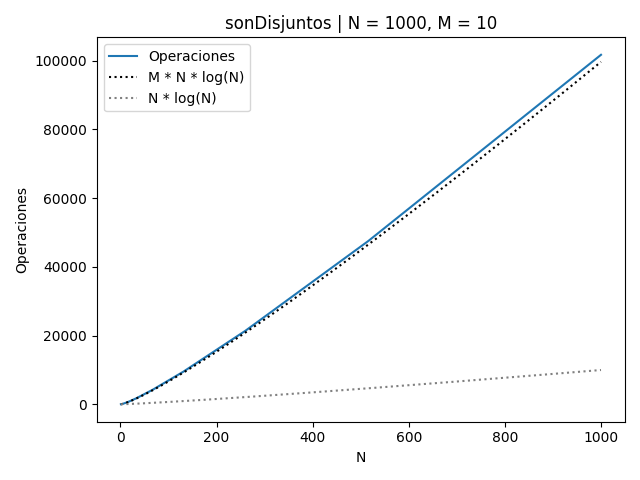
\includegraphics[width=\linewidth]{img/sonDisjuntos_1000_10}
  \endminipage\hfill
  \minipage{0.32\textwidth}
    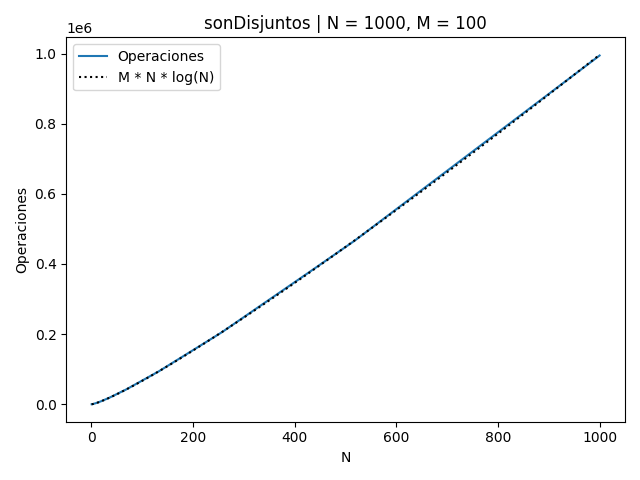
\includegraphics[width=\linewidth]{img/sonDisjuntos_1000_100}
  \endminipage\hfill
  \minipage{0.32\textwidth}%
    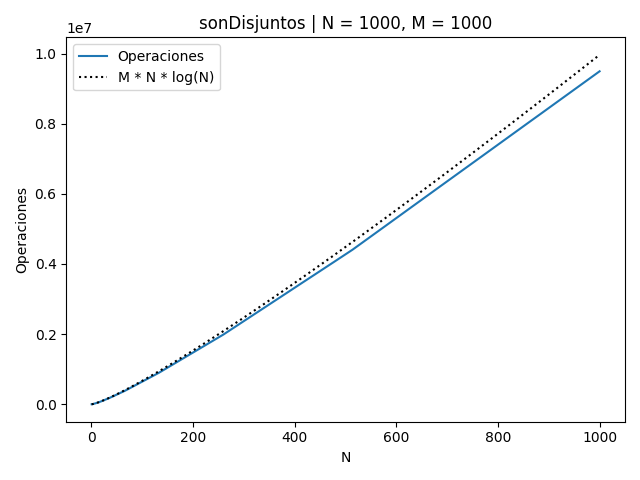
\includegraphics[width=\linewidth]{img/sonDisjuntos_1000_1000}
  \endminipage
\end{figure}

Como se puede notar en los gr\'aficos, la cantidad de operaciones que realiza el algoritmo est\'a en el orden de $\bigO(M \cdot N \cdot \log N)$ y adem\'as, al aumentar el $M$ multiplicando por 10, se puede ver que la cantidad de operaciones tambi\'en se multiplica por 10.

\vspace{0.5em}

El c\'odigo, datos y gr\'aficos se encuentran en las carpetas \texttt{scripts}, \texttt{data} e \texttt{img}.

% \newpage

\vspace{1em}

\textbf{2. (optativo)} Suponiendo que los elementos de todos los conjuntos est\'an en el rango comprendido entre 1 y el producto $M \cdot N$, proponer un algoritmo para resolver el mismo problema con complejidad temporal en peor caso $O(M \cdot N)$. Notar que este algoritmo sirve para determinar si los conjuntos $C[1],...,C[N]$ constituyen una partici\'on del conjunto $\{1, 2,..., M \cdot N - 1, M \cdot N\}$. Justificar la complejidad temporal obtenida

\vspace{0.5em}

\textbf{Idea: }
\begin{enumerate}
  \item Al estar los conjuntos acotados entre $1$ y $M \cdot N$, para que los conjuntos sean disjuntos dos a dos, entonces debe ocurrir que todos los naturales entre $1$ y $M \cdot N$ est\'en comprendidos en la lista de conjuntos.
  \item Haciendo un tipo de counting sort para ver si todos los elementos entre $1$ y $M \cdot N$ est\'an en la uni\'on de todos los conjuntos podemos determinar si son disjuntos dos a dos.
  \item Esto se debe a que si no est\'an todos los elementos, entonces debe ocurrir que alg\'un natural est\'a repetido en alg\'un conjunto ya que los conjuntos tienen todos exactamente $M$ elementos y el total de elementos es $M \cdot N$.
\end{enumerate}

\textbf{Algoritmo: }
\begin{enumerate}
  \item Nos generamos un \texttt{vector(bool)} de tama\~no $M \cdot N$ inicializado con todo en $false$.
  \item Iteramos por todos los elementos de todos los conjuntos, y por cada natural, seteamos en $true$ su aparici\'on en el vector generado anteriormente. Particularmente le restamos 1 a cada valor ya que los valores van entre $1$ y $M \cdot N$ mientras que los \'indices de nuestro arreglo est\'an entre $0$ y $M \cdot N - 1$.
  \item Una vez seteado todos los valores en $true$ de los elementos que se encuentran, resta revisar que ning\'un valor sea $false$, ya que en ese caso ese n\'umero no estar\'ia en ning\'un conjunto, lo cual implica que hay alguno con repetidos y no ocurrir\'a que todos sean disjuntos dos a dos.
  \item Si todos los n\'umeros estaban en los conjuntos entonces el vector tiene todos los valores en $true$ y retornamos que son disjuntos dos a dos.
\end{enumerate}

\begin{algorithm}[H]
	\caption{\textbf{sonDisjuntosAcotado}(\In{A}{vector(conj(nat))}, \In{m}{nat}) $\to$ $res$ : \texttt{bool}}
	\begin{algorithmic}[1]
    \State \asignar{n}{Longitud(A)}
    \State \asignar{nm}{n \times m}
    \State \asignar{countingVec}{Vacia()}
    \State \asignar{i}{0}
    \For{$i < nm$} \Comment{$\bigO(M \cdot N)$}
      \State $AgregarAtras(countingVec, false)$ \Comment{$\bigO(1)$}
      \State \asignar{i}{i + 1}
    \EndFor

    \State \asignar{i}{0}
    \For{$i < n$} \Comment{$\bigO(M \cdot N)$}
      \For{$a$ \textbf{in} $A[i]$} \Comment{$\bigO(M)$}
        \State \asignar{countingVec[a - 1]}{true} \Comment{$\bigO(1)$}
      \EndFor
      \State \asignar{i}{i + 1}
    \EndFor

    \State \asignar{i}{0}
    \For{$i < nm$} \Comment{$\bigO(M \cdot N)$}
      \If{$countingVec[i] = false$}
        \State \Return{false}
      \EndIf
      \State \asignar{i}{i + 1}
    \EndFor

    \State \Return{true}
		\medskip
	\end{algorithmic}
\end{algorithm}

\textbf{Complejidad: }
\begin{enumerate}
  \item Generar un vector de tama\~no $M \cdot N$ con todos los elementos en $false$ nos cuesta $\bigO(M \cdot N)$.
  \item Iterar por todos los elementos de todos los conjuntos tamb\'ien nos cuesta $\bigO(M \cdot N)$. Setear un \'indice en $true$ tiene costo $\bigO(1)$.
  \item Finalmente, iterar nuevamente por el vector nos cuesta en peor caso $\bigO(M \cdot N)$ ya que ocurre cuando todos los valores est\'en en $true$ y sean conjuntos disjuntos dos a dos.
\end{enumerate}

Luego, queda demostrado que para conjuntos acotados, \textsc{sonDisjuntosAcotado} $\in \bigO(M \cdot N)$. $\blacksquare$

\end{document}
